In a game of \textit{Chomp}, two players alternately take bites from a 5-by-7 grid of unit squares. To take a bite, a player chooses one of the remaining squares, then removes ("eats'') all squares in the quadrant defined by the left edge (extended upward) and the lower edge (extended rightward) of the chosen square. For example, the bite determined by the shaded square in the diagram would remove the shaded square and the four squares marked by $\times.$ (The squares with two or more dotted edges have been removed form the original board in previous moves.)

\begin{center}
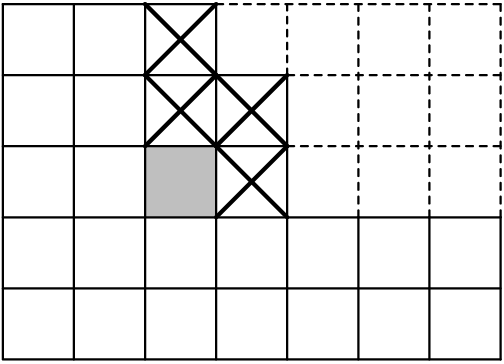
\includegraphics[width = 50.400000000000006mm]{img/fig0.png}
\end{center}

The object of the game is to make one's opponent take the last bite. The diagram shows one of the many subsets of the set of 35 unit squares that can occur during the game of Chomp. How many different subsets are there in all? Include the full board and empty board in your count.